\section{Ejercicios}

\begin{enumerate}

\item En el circuito de la figura, el interruptor ha estado abierto durante un tiempo
prolongado, y en el instante $t = 0$ se cierra. Se debe determinar el valor de las tensiones y corrientes del circuito en $t = 0^+$.

\begin{minipage}{0.5\linewidth}
  \center{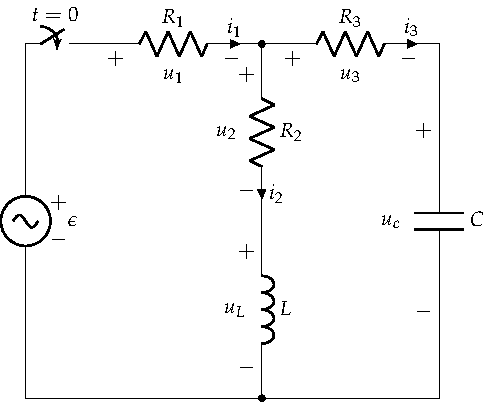
\includegraphics{../figs/BT4_CondicionesIniciales_bobcon.pdf}}
\end{minipage}
\begin{minipage}{0.5\linewidth}
  \center{Datos:}
  \begin{align*}
    R_1 &= 3\,\unit{\ohm}\\
    R_2 &= 5\,\unit{\ohm}\\
    R_3 &= 2\,\unit{\ohm}\\
    L &= 0.2\,\unit{\henry}\\
    C &= 0.5\,\unit{\milli\farad}\\
    \epsilon(t) &= 20\cos(t)\unit{\volt}
  \end{align*}
\end{minipage}

\vspace{2mm}
\emph{Sol.:\;   $i_1(0^+) = i_3(0^+) = \qty{4}{\ampere}$;\; 
  $u_1(0^+) = \qty{12}{\volt}$;\;
  $u_2(0^+) = \qty{0}{\volt}$;\;
  $u_3(0^+) = \qty{8}{\volt}$;\;
  $u_L(0^+) = u_3(0^+) = \qty{8}{\volt}$
}

\item El interruptor de la figura lleva cerrado un tiempo que se puede
  considerar infinito. En el instante $t=0$, se abre, permaneciendo en
  esta posición definitivamente. Calcular la expresión de la
  intensidad $i(t)$ desde $t=0$ en adelante.  
  
  Datos:\;
  $E = \qty{1}{\volt}$;\; $R_1 = \qty{1}{\ohm}$;\;
  $R_2 = R_3 = \qty{2}{\ohm}$;\; $C = \qty{4}{\milli\farad}$

  \begin{center}
    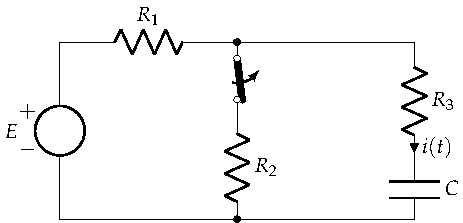
\includegraphics{../figs/BT4_01.pdf}
  \end{center}

  \emph{Sol.:\; $i(t)=\dfrac{1}{9}\; \mathrm{e}^{-\frac{t}{0.012}} \;\si{\ampere}$}
  
\item El circuito de la figura se encuentra en régimen permanente. En
  el instante $t=0$ se abre el interruptor. Calcular $u_1$ y $u_2$
  para $t>0$.

  Datos:\; $E = \qty{15}{\volt}$;\; $R_1 = \qty{200}{\ohm}$;\;
  $R_2 = \qty{100}{\ohm}$;\; $C_1 = \qty{2}{\micro\farad}$;\;
  $C_2 = \qty{4}{\micro\farad}$

  \begin{center}
    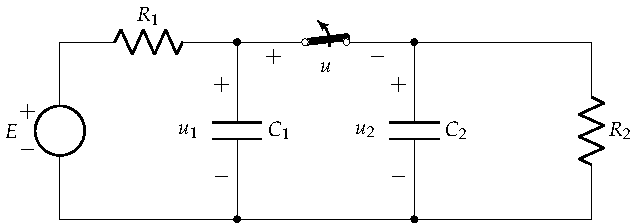
\includegraphics{../figs/BT4_02.pdf}
  \end{center}

  \emph{Sol.:\;
    $u_1(t)=15-10\cdot\mathrm{e}^{-2500\,t}\;\si{\volt};\;
    u_2(t)=5\cdot\mathrm{e}^{-2500\,t}\;\si{\volt}$}
  
\item El interruptor del circuito de la figura lleva cerrado un timepo
  que se considera infinito. En el instante $t=0$, se abre y permanece
  en dicha posición definitivamente. Hállese la expresión de $u(t)$ e
  $i(t)$ para $t>0$.

  Datos:\; $E = \qty{36}{\volt}$;\; $R_1 = \qty{2}{\ohm}$;\;
  $R_2 = \qty{4}{\ohm}$; $R_3 = \qty{3}{\ohm}$;\;
  $C = \qty{3}{\milli\farad}$; $L = \qty{6}{\milli\henry}$

\begin{center}
  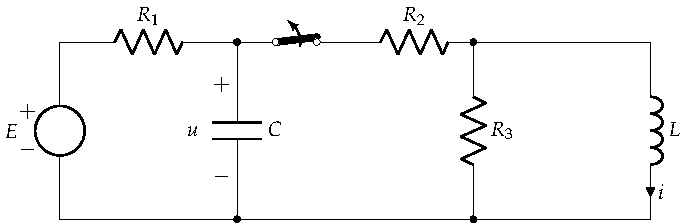
\includegraphics{../figs/BT4_03.pdf}
\end{center}

\emph{Sol.:\;
  $u(t)=36-12\cdot\mathrm{e}^{-166.67\,t}\;\si{\volt};\;
  i(t)=6\cdot\mathrm{e}^{-500\,t}\;\si{\ampere}$}

\item El circuito de la figura lleva en esa posición un tiempo que se
  puede considerar infinito. En el instante $t=0$, ambos interruptores
  cambian su posición. Calcular la expresión de $u(t)$ para $t>0$.

  Datos:\; $E_1 = \qty{40}{\volt}$;\; $R_1 = \qty{20}{\ohm}$;\;
  $R_2 = \qty{60}{\ohm}$;\; $R_3 = \qty{3}{\ohm}$;\;
  $R_4 = \qty{6}{\ohm}$;\; $C = \qty{0.5}{\milli\farad}$;\;
  $e_2(t) = 120 \, \cos(1000t)\unit{\volt}$

  \begin{center}
    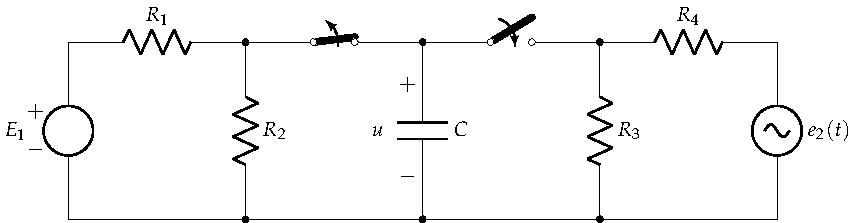
\includegraphics{../figs/BT4_04.pdf}
  \end{center}

  \emph{Sol.:\;
    $u(t)=10\cdot\mathrm{e}^{-1000\,t}+20\sqrt{2}\,\cos\left(1000\,t-\frac{\pi}{4}\right)\;\si{\volt}$}

\item En el circuito de la figura se abre el interruptor después de un
  tiempo suficientemente grande para considerar que el circuito
  funcionaba en régimen permanente. Expresar las formas de onda de
  $i_1$, $i_2$ y $u_L$ para $t>0$.

  Datos:\; $e(t)=220\sqrt{2}\,\cos(100\pi\,t)\,\unit{\volt}$;\;
  $L = \qty{0.2}{\henry}$;\; $R_1 = \qty{25}{\ohm}$;\;
  $R_2 = \qty{275}{\ohm}$

  \begin{center}
    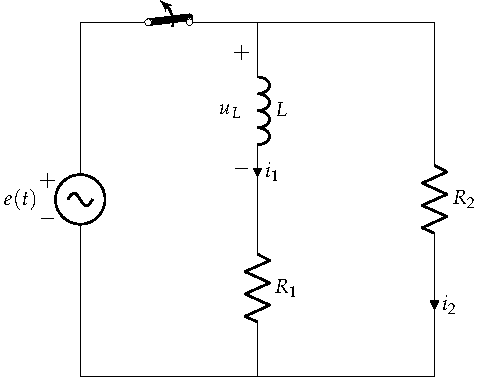
\includegraphics{../figs/BT4_05.pdf}
  \end{center}

  \emph{Sol.:\;
    $i_1(t)=1.7\cdot\mathrm{e}^{-1500\,t}\;\si{\ampere};\; i_2(t)=-1.7\cdot\mathrm{e}^{-1500\,t}\;\si{\ampere};\;
    u_L(t)=-510\cdot\mathrm{e}^{-1500\,t}\;\si{\volt}$}

\item En el circuito de la figura, en $t = 0$ se cierra el
  interruptor. Obtener la expresión analítica de la intensidad $i(t)$,
  para $t > 0$.

  Datos:\; $E = \qty{10}{\volt}$;\; $L = \qty{0.2}{\henry}$;\;
  $I_g = \qty{1}{\ampere}$;\; $R_1 = \qty{10}{\ohm}$;\;
  $\alpha = \qty{3}{\ohm}$

  \begin{center}
    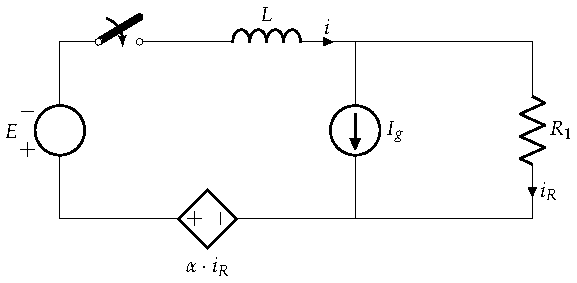
\includegraphics{../figs/BT4_06.pdf}
  \end{center}

    \vspace*{-7mm}
  \emph{Sol.:\; $i(t)=\dfrac{3}{7}\,(\mathrm{e}^{-35\,t}-1) \;\si{\ampere}$}
  

\item El interruptor de la figura ha estado cerrado por un tiempo
  prolongado y en $t = 0$ se abre.

\begin{minipage}{0.5\linewidth}
  \center{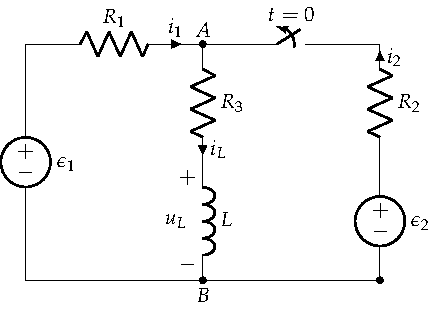
\includegraphics{../figs/BT4_CondicionesIniciales_bobina.pdf}}
\end{minipage}
\begin{minipage}{0.5\linewidth}
  \hspace{20mm} Datos:
  \begin{align*}
    R_1 &= \SI{5}{\ohm}\\
    R_2 &= \SI{5}{\ohm}\\
    R_3 &= \SI{2}{\ohm}\\
    L &= \SI{3.5}{\milli\henry}\\
    \epsilon_1 &= \SI{24}{\volt}\\
    \epsilon_2 &= \SI{12}{\volt}
  \end{align*}
\end{minipage}

\medskip

Con esta información, se debe calcular:
\begin{enumerate}
\item Valores de $i_1(0^+)$, $i_2(0^+)$, $i_L(0^+)$, $u_L(0^+)$ y
  $u_{AB}(0^+)$.
\item Expresión de $i_L(t)$ para $t > 0$.
\item Expresiones de $u_L(t)$ y $u_{AB}(t)$ para $t > 0$.
\end{enumerate}

\vspace{2mm}
\emph{Sol.:\; $i_L(t) = 3.43 + 0.57 \cdot e^{-2000 \cdot t} \;\unit{\ampere}$;\;
  $u_L(t) = - 4 \cdot e^{-2000 \cdot t} \;\unit{\volt}$;\;
  $u_{AB}(t) = 6.86 - 2.86 \cdot e^{-2000 \cdot t} \;\unit{\volt}$
}

\item El interruptor del circuito de la figura lleva abierto un tiempo
  indefinido. En el instante $t= 0$ se cierra este interruptor. Hay
  que obtener:
  \begin{enumerate}
  \item Valores de las tensiones $u_1(0^+)$, $u_2(0^+)$, $u_3(0^+)$ y
    $u_c(0^+)$.
  \item Expresión temporal de la tensión $u_c(t)$ para $t > 0$.
  \item Expresiones temporales de $u_2(t)$ y $u_3(t)$ para $t > 0$.
  \end{enumerate}

\begin{minipage}{0.5\linewidth}
  \center{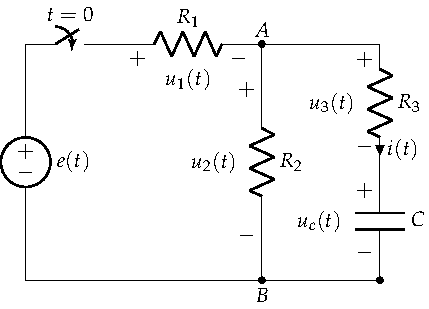
\includegraphics{../figs/BT4_CondicionesIniciales_condensador.pdf}}
\end{minipage}
\begin{minipage}{0.5\linewidth}
 \hspace{20mm} Datos:
    \begin{align*}
    e(t) &= 10\,\unit{\volt}\\
    R_1 &= R_2 = 2 \,\unit{\ohm}\\
    R_3 &= 4 \,\unit{\ohm}\\
    C &= 1 \,\unit{\farad}
  \end{align*}
\end{minipage}

\emph{Sol.:\; $u_c(t) = 5 \cdot(1 - e^{-0.2t}) \;\unit{\volt}$;\;
  $u_2(t) = 5 - e^{-0.2t} \;\unit{\volt}$;\;
  $u_3(t) = 4 \cdot e^{-0.2t} \;\unit{\volt}$}

\item Calcular la corriente $i(t)$ para $t > 0$.

\begin{minipage}{0.5\textwidth}
  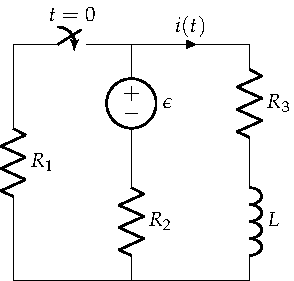
\includegraphics{../figs/FM_4_2}
\end{minipage}
\hfill
\begin{minipage}{0.5\textwidth}
  Datos:
  \begin{align*}
    \epsilon &= \SI{24}{\volt}\\
    R_1 &= \SI{8}{\ohm}\\
    R_2 &= \SI{4}{\ohm}\\
    R_3 &= \SI{4}{\ohm}\\
    L &= \SI{15}{\henry}
  \end{align*}
\end{minipage}

\vspace{2mm}
\emph{Sol.:\; $i(t) = 0.6 \cdot e^{-4t/9} + 2.4 \;\si{\ampere}$}

\item Calcular la tensión en bornes del condensador para $t > 0$.

\begin{minipage}{0.5\textwidth}
  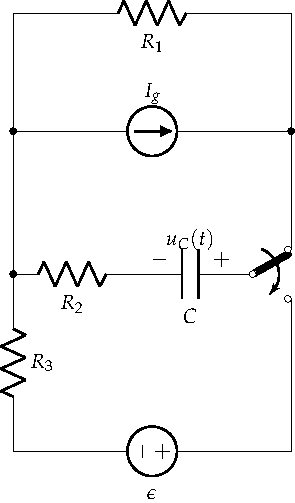
\includegraphics[scale=0.85]{../figs/FM_4_3}
\end{minipage}
\hfill
\begin{minipage}{0.5\textwidth}
  Datos:
  \begin{align*}
    \epsilon &= \SI{20}{\volt}\\
    I_g &= \SI{4}{\ampere}\\
    R_1 &= \SI{6}{\ohm}\\
    R_2 &= \SI{4}{\ohm}\\
    R_3 &= \SI{12}{\ohm}\\
    C &= \SI[parse-numbers=false]{1/16}{\farad}      
  \end{align*}

\end{minipage}

\vspace{2mm}
\emph{Sol.:\; $u_C(t) = 4 \cdot e^{-t} + 20 \;\si{\volt}$}

\item Determina las corrientes $i_L(t)$ e $i_1(t)$ para $t > 0$.

\begin{minipage}{0.7\textwidth}
  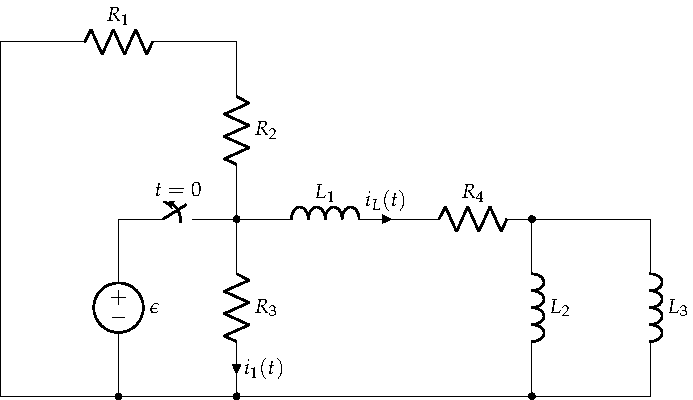
\includegraphics{../figs/HKD84}
\end{minipage}
\hfill
\begin{minipage}{0.3\textwidth}
  Datos:
  \begin{align*}
    \epsilon &= \SI{18}{\volt}\\
    R_1 &= \SI{120}{\ohm}\\
    R_2 &= \SI{60}{\ohm}\\
    R_3 &= \SI{90}{\ohm}\\
    R_4 &= \SI{50}{\ohm}\\
    L_1 &= \SI{1}{\milli\henry}\\
    L_2 &= \SI{2}{\milli\henry}\\
    L_3 &= \SI{3}{\milli\henry}
  \end{align*}
\end{minipage}

\vspace{2mm}
\emph{Sol.:\; $i_L(t) = 0.36 \cdot e^{-5 \cdot 10^{4} \cdot t}\;\si{\ampere}$;\;
  $i_1(t) = -0.24 \cdot e^{-5 \cdot 10^{4} \cdot t} \;\si{\ampere}$}

\item El circuito de la figura ha alcanzado el régimen permanente con
  el interruptor cerrado. El interruptor se abre en $t = 0$. Calcula
  las expresiones de la tensión en bornes del condensador y de la
  corriente por la bobina para $t > 0$.

  \vspace{2mm}

\begin{minipage}{0.7\textwidth}
  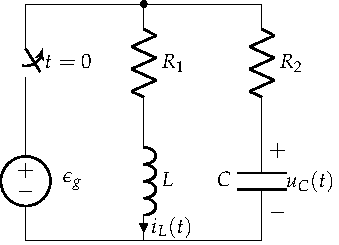
\includegraphics[scale=0.95]{../figs/FM_4_8}
\end{minipage}
\hfill
\begin{minipage}{0.3\textwidth}
  Datos:
  \begin{align*}
    \epsilon_g &= \SI{10}{\volt}\\
    R_1 &= \SI{10}{\ohm}\\
    R_2 &= \SI{5}{\ohm}\\
    L &= \SI{2.5}{\henry}\\
    C &= \SI{0.2}{\farad}      
  \end{align*}
\end{minipage}

\vspace{2mm}
\emph{Sol.:\; $i_L(t) = 0.689 \cdot e^{-0.354 \cdot t} + 0.311 \cdot e^{-5.645 \cdot t} \;\si{\ampere}$;\;
$u_C(t) = 9.7275 \cdot e^{-0.354 \cdot t} + 0.275 \cdot e^{-5.645 \cdot t} \;\si{\volt}$}

\item En el circuito de la figura calcular la tensión $u_C(t)$ para
  $t > 0$.

  \begin{minipage}{0.5\linewidth}
    \begin{center}
      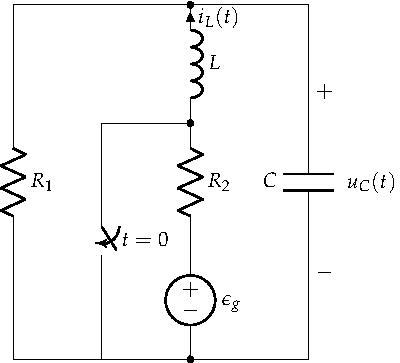
\includegraphics{../figs/FM_4_9.pdf}
    \end{center}
  \end{minipage}
  \begin{minipage}{0.5\linewidth}

    \center{Datos:}
  \begin{align*}
    \epsilon_g &= \SI{4}{\volt}\\
    R_1 &= \SI{2}{\ohm}\\
    R_2 &= \SI{2}{\ohm}\\
    L &= \SI{1}{\henry}\\
    C &= \SI{0.25}{\farad}      
  \end{align*}
  \end{minipage}

  \emph{Sol.:\;
    $u_C(t)=
    \mathrm{e}^{-t}\left[2\,\cos(\sqrt{3}\,t)+\dfrac{2}{\sqrt{3}}\,\sin(\sqrt{3}\,t)\right]=\dfrac{4\sqrt{3}}{3}\,\mathrm{e}^{-t}\,\sin\left(\sqrt{3}\,t+\dfrac{\pi}{6}\right) \;\si{\volt}$
    }

\item En el circuito de la figura el interruptor ha estado cerrado
  durante un tiempo elevado, y en $t = 0$ se abre. En estas
  condiciones se debe determinar:

  \begin{enumerate}
  \item Tipo de transitorio presente en el circuito.

  \item Condiciones iniciales de las siguientes variables del
    circuito: $u_C(0^+)$, $i_L(0^+)$, $i_C(0^+)$, $u_L(0^+)$.
  \item Valores en régimen permanente de las siguientes variables del
    circuito: $u_C(\infty)$, $i_L(\infty)$, $i_C(\infty)$,
    $u_L(\infty)$.
  \item Expresión de la corriente $i_L(t)$ para $t > 0$.
  \item Expresión de la tensión $u_C(t)$ para $t > 0$.
  \end{enumerate}

\begin{minipage}{0.3\linewidth}
  Datos:
    \vspace{2mm}

  $E_g = \SI{500}{\volt}$

  $R_{1}= \SI{375}{\ohm}$%

  $R_{2}=\SI{125}{\ohm}$%

  $L_1 = \SI{40}{\milli\henry}$%

  $C = \SI{1}{\micro\farad}$%
\end{minipage}
\begin{minipage}{0.7\linewidth}
  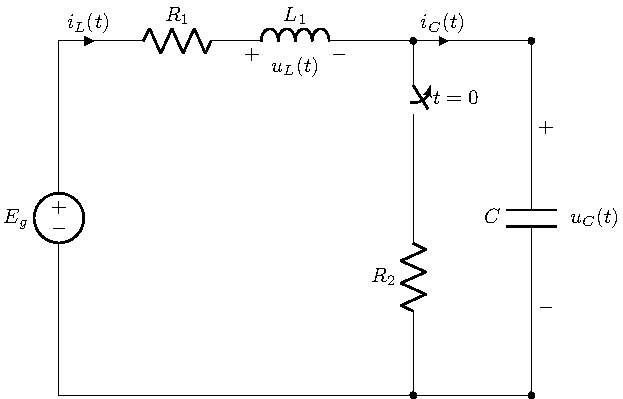
\includegraphics{../figs/E1_RLC.pdf}
\end{minipage}

\emph{Sol.:\;\;
  $i_L(t)=
  \mathrm{e}^{-4687.5\,t}\left[\cos(1740\,t)+2.7\,\sin(1740\,t)\right]=2.88\,\mathrm{e}^{-t}\,\sin\left(1740\,t+0.3547\right)\;\unit{\ampere}$;\;\;
  $u_C(t) = 500 - e^{-4687.5 \,t} \left[435.9\, \sen(1740 \,t) + 375\, \cos(1740 \,t)\right] = 500 - 575.01 \cdot e^{-4687.5 \,t} \cdot  \sen(1740 \,t + 0.7104)\;\unit{\volt}$
  }

\end{enumerate}
%%% Local Variables:
%%% mode: latex
%%% TeX-master: "enunciados_ejercicios_TC"
%%% ispell-local-dictionary: "castellano"
%%% End:
